\par Data used for this analysis was collected by the ATLAS detector during Run II 
of the LHC. The LHC parameters and conditions during this data-taking period are discussed 
in Chapter~\ref{expSetup}. Only data from runs during which proton beams were stable\footnote{Stable beams 
are those that have a stable energy of 6.5~\TeV.} were considered. 
The total integrated luminosity of this data-set is 14.7~\ifb, 3.2~\ifb\ of 
which was collected in 2015. The rest was collected in 2016. Uncertainties on the 2016 
and 2015 luminosities were 3.7\% and 2.1\% respectively. The impact of these uncertainties on the 
final results of this search is discussed in Section~\ref{sec:resCh}. 

\par Expected signal and background events were computed using Monte Carlo (MC) simulation, 
as discussed in detail in Chapter~\ref{sim}. 
%Ingredients for such simulations are 
%\begin{enumerate}
%\item a hard scatter event generator;
%\item a set of parton density functions (PDFs) that describe momentum distributions of gluons and quarks 
%in the proton; 
%\item an underlying event generator that is tuned to match conditions during data-taking period;
%\item and models for parton showering, fragmentation and hadronization that are also tuned to match real data. 
%\end{enumerate} 
%
As discussed in Section~\ref{sec:cHtheory}, 
for high \mcH\ the charged Higgs boson is produced in association with a top quark. Such a production mode 
is dominated by the 4FS and 5FS diagrams shown in Figure~\ref{fig:chargedFeynV1}.
 Since the 4FS and 5FS diagrams have similar topologies~\cite{Flechl:2014wfa},  
without loss of generality signal samples were generated only from the 4FS diagram. 
Using the NNPDF23LO~\cite{Ball:2012cx} PDF set, hard scatter 
events were generated by \MGMCatNLO~\cite{Alwall:2014hca} version 2.2.2.
Underlying events were generated by \PYTHIA8~\cite{Pythia8} version 8.186,
 whose parameters were tuned to match parameters, 
called A14~\cite{ATL-PHYS-PUB-2014-021}, observed in data. 
Parton showering, fragmentation and hadronization were handled 
by \PYTHIA~\cite{Sjostrand:2000wi} version 6.428. 
Taking the mass of the top quark as $172.5~\GeV$,  
18 signal samples with $200~\GeV\leq\mcH\leq2000~\GeV$ were independently generated.   

\begin{figure}[!h]
\centering
\begin{subfigure}{0.4\textwidth}
   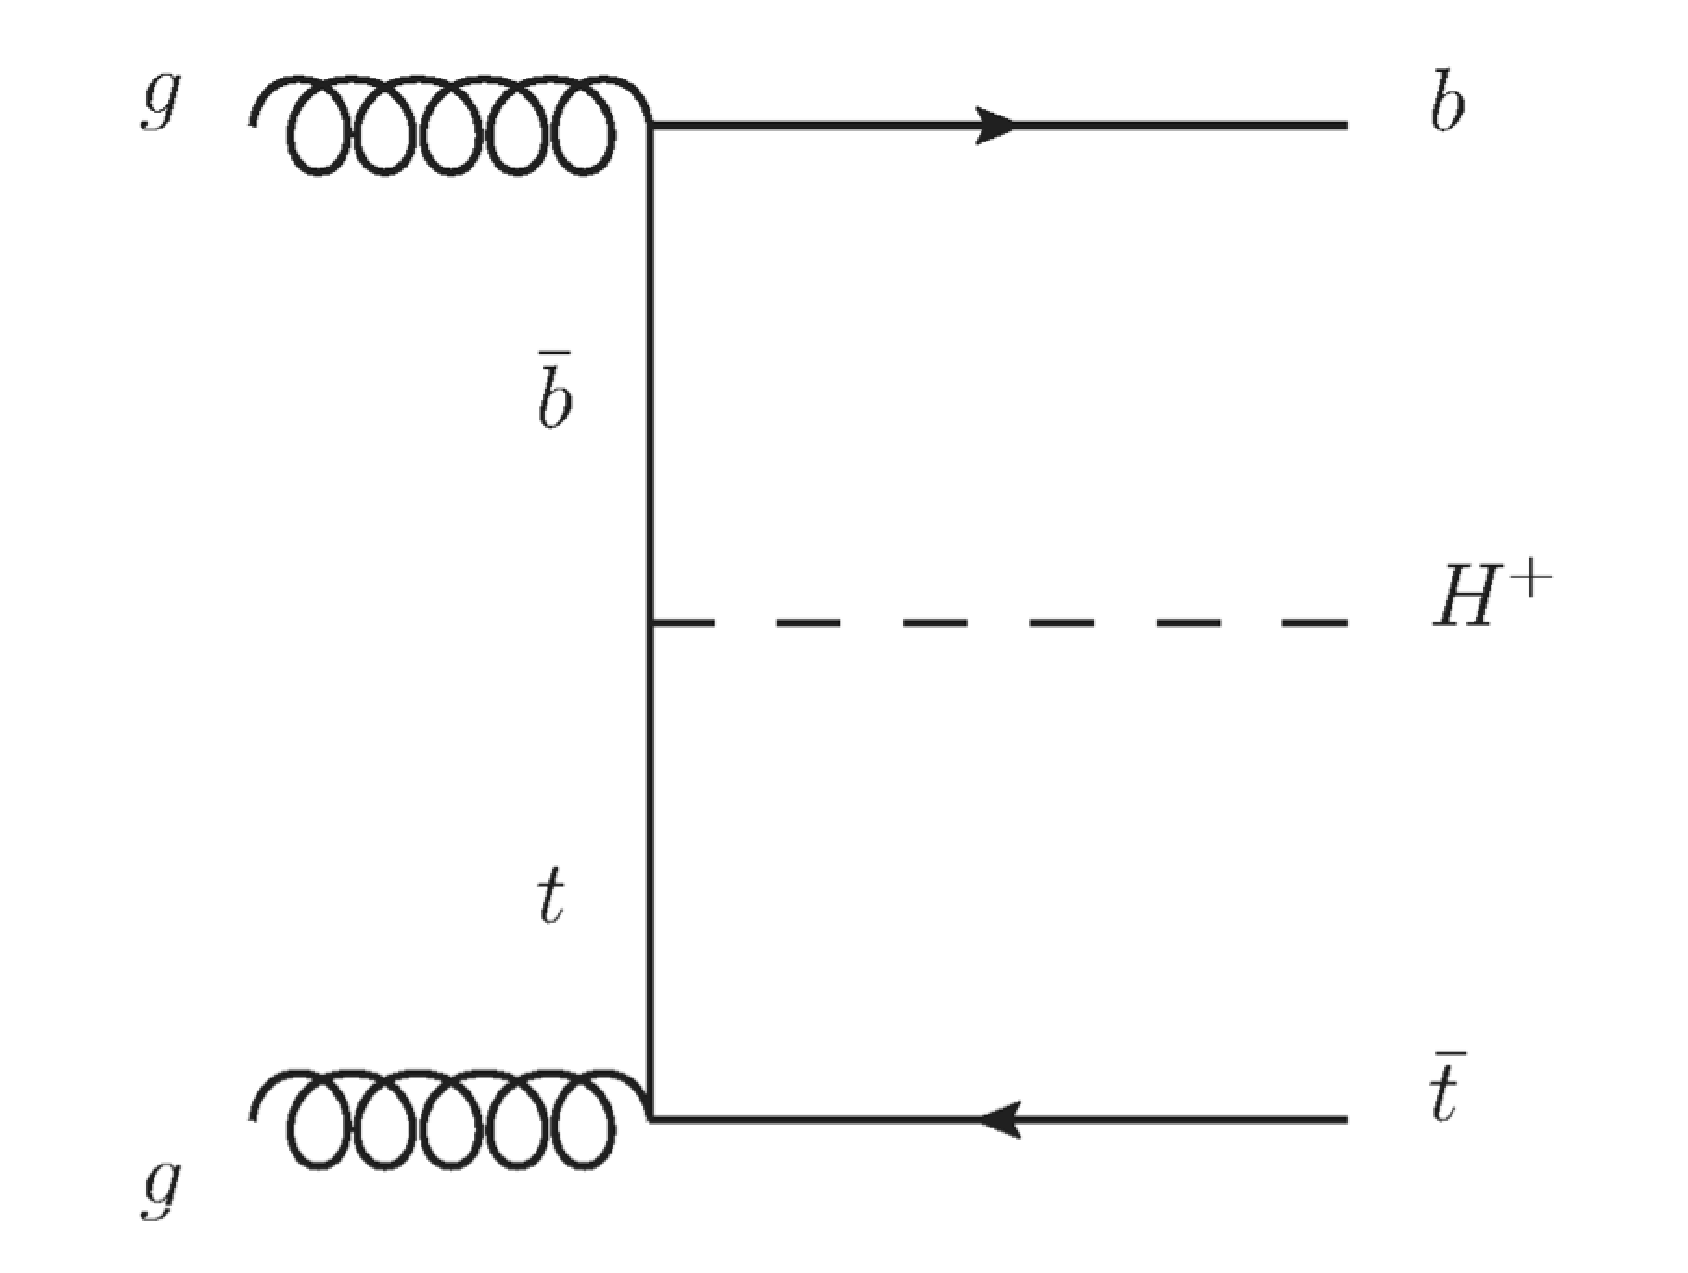
\includegraphics[width=\textwidth]{figures/feynmanIIIa.eps}
\caption{Top association -- 4FS}
\end{subfigure} % 
\begin{subfigure}{0.4\textwidth}
   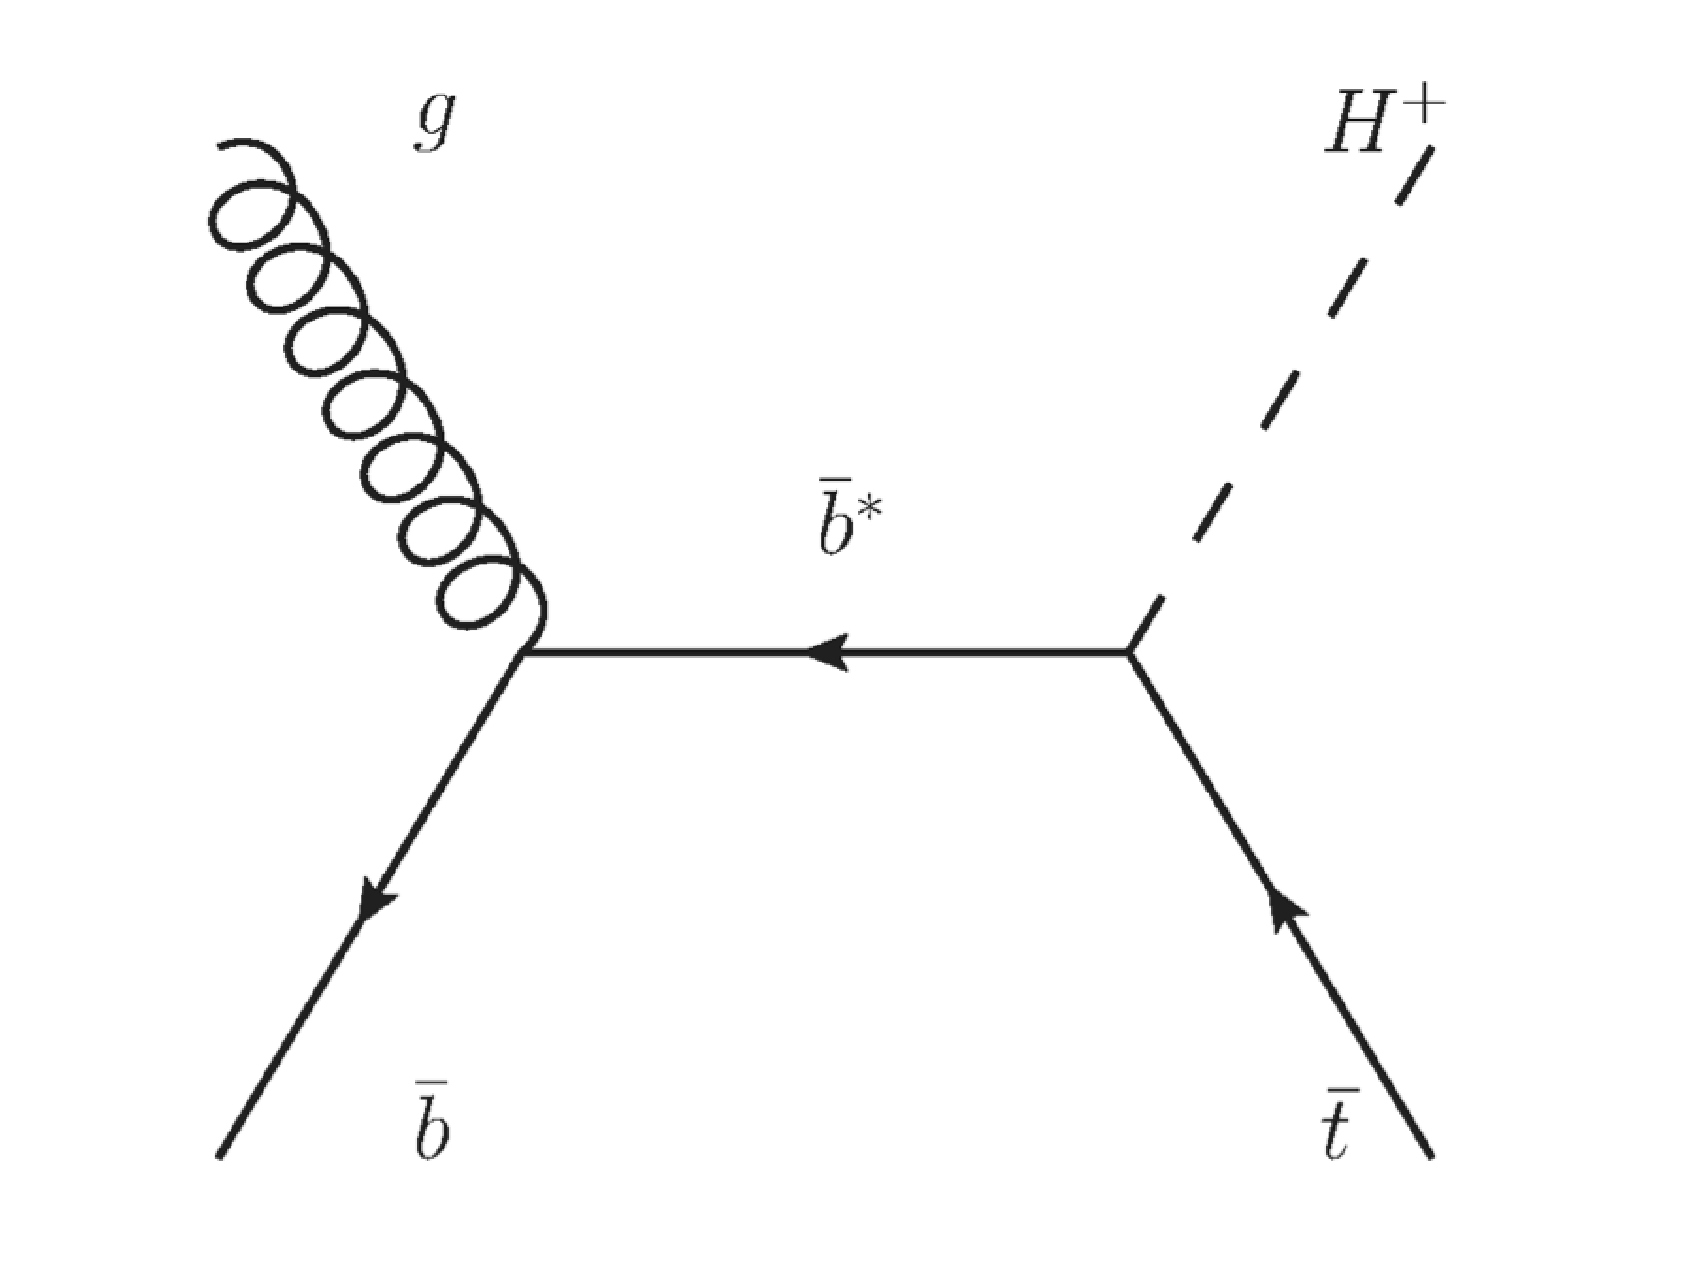
\includegraphics[width=\textwidth]{figures/feynmanIIa.eps}
\caption{Top association -- 5FS}
\end{subfigure} %
\caption{Leading order Feynman diagrams for the charged Higgs boson production}
\label{fig:chargedFeynV1}
\end{figure}

\par The \ttbar\ process, shown in Figure~\ref{fig:ttBarDg}, is the most dominant process 
with a top quark in the final state at the 
LHC~\cite{Aad:2015eia}. It is therefore expected to be the most dominant background to the charged Higgs boson 
produced in association with a top quark.
The next dominant source of top quarks at the LHC is the {\it single top} process, 
produced through any of the $\operatorname{s-,t-}$ or $\operatorname{Wt-}$channels shown in Figure~\ref{fig:singleTopDg}.
The hard scatter events for \ttbar, $\operatorname{Wt-}$ and $\operatorname{s-}$channel single top processes 
were generated by \POWHEG-\textsc{Box}~\cite{PowhegBox, Alioli:2008tz,Powheg0,Powheg1,Powheg2} version 2
 at NLO, using the CT10~\cite{Lai:2010vv, Gao:2013xoa} PDF set.  
\POWHEG-\textsc{Box} version 1 was used to generate the $\operatorname{t-}$channel single top hard scatter event, 
using the CT10F4\footnote{The `F4' indicates that this is a 4FS version of the standard CT10 PDF set}
 PDF set. Again, the mass of the top quark was set at $172.5~\GeV$. 
Using the CTEQ6L1~\cite{Nadolsky:2008zw} PDF set \PYTHIA\ version 6.428 was used to model parton showering, 
fragmentation and the underlying event. These models were tuned with the Perugia 2012~\cite{Skands:2010ak} parameters. 
While the \ttbar\ cross section was calculated to NNLO+NNLL, 
single top processes were normalized to NNLO cross sections.   

\par \ttbar\ and single top processes are collectively referred to in this search 
as {\it Top}.\footnote{Not to be confused with the {\it top} quark, which will either be 
in full small caps, or abbreviated to $t$.}

\begin{figure}[h]
   \includegraphics[width=.5\textwidth]{figures/feynman_ttbar_LHC_gggtt.png}
   \includegraphics[width=.5\textwidth]{figures/feynman_ttbar_LHC_ggttt.png}
\caption{Leading order Feynman diagrams for \ttbar\ production at the LHC. Taken from 
Ref~\cite{D0:ttBarFeyn}}
\label{fig:ttBarDg}
\end{figure} % 

\begin{figure}[h]
\begin{subfigure}{0.33\textwidth}
					 \includegraphics[width=\textwidth]{figures/feynman_tb_bold_ltblue_whitebkgd.png}
\caption{$\operatorname{s-}$channel}
\end{subfigure}%  
\begin{subfigure}{0.33\textwidth}
					 \includegraphics[width=\textwidth]{figures/feynman_tq_bold_midblue.png}
\caption{$\operatorname{t-}$channel}
\end{subfigure}%
\begin{subfigure}{0.33\textwidth}
					 \includegraphics[width=\textwidth]{figures/feynman_tqb_bb_bold_midblue.png}
\caption{$\operatorname{Wt-}$channel}
\end{subfigure}%
\caption{Leading order Feynman diagrams for single top quark production at the LHC. Taken 
from Ref~\cite{D0:ttBarFeyn}} 
\label{fig:singleTopDg}
\end{figure} % 

\par Events containing a $W$ or \Zboson\ boson and some associated jets are 
also expected to be a significant background to the signal. Their hard scatter events were generated by 
\MGMCatNLO\ version 2.2.2 with the NNPDF23LO PDF set. \PYTHIA8\ was used to generate 
the underlying events, while \PHOTOS~\cite{Davidson:2010ew} was used to radiate photons from charged leptons. 
All the cross sections were normalized to NNLO. 

\par Events with two vector bosons and associated
jets, referred to collectively as {\it VV} or {\it Diboson}, were generated by \POWHEG-\textsc{Box} version 2 interfaced 
with \PYTHIA\ version 8.186 for the parton shower models. The CT10 PDF set was used to model 
gluon and quark momenta in the protons. Cross sections were normalized to NLO. 

\par Bottom and charm quark decays were produced and decayed by \textsc{Evtgen}~\cite{Lange2001152}
 version 1.2.0. Pileup events were added to these 
events with \PYTHIA\ version 8 using the MSTW2008LO~\cite{Martin:2009iq, Martin:2009bu, Martin:2010db}
 PDF set. Just like in signal, parton showering, hadronization and fragmentation models in \PYTHIA\ version 8 were 
also tuned with the A14 parameter set.  
